\documentclass[aspectratio=169]{beamer}

% --- TEMASI VE RENKLER ---
\usetheme{Madrid}
\usecolortheme{whale}

% Ozel renkler (NexOS temasi - Koyu Mavi/Cyan)
\definecolor{NexosDark}{RGB}{10, 30, 60}
\definecolor{NexosCyan}{RGB}{0, 150, 200}

\setbeamercolor{structure}{fg=NexosDark}
\setbeamercolor{frametitle}{bg=NexosDark, fg=white}
\setbeamercolor{title}{bg=NexosDark, fg=white}

% --- PAKETLER ---
\usepackage[utf8]{inputenc}
\usepackage[T1]{fontenc}
\usepackage{graphicx}
\usepackage{tikz}
\usepackage{listings}

% --- TIKZ AYARLARI (Mimari semasi icin) ---
\usetikzlibrary{shapes,arrows,positioning}

% --- BILGILER ---
\title[NexOS]{NexOS: Yeni Nesil Eğitim İşletim Sistemi}
\subtitle{Kapsamlı Teknik Sunum}
\author[M. Omar \& A. R. Mistik]{
    MASIHULLAH OMAR (170422921)\\
    ALİ RIZA MISTIK (170423851)
}
\institute{Bilgisayar Mühendisliği}
\date{30 Aralık 2025}

% --- LOGO ---
\titlegraphic{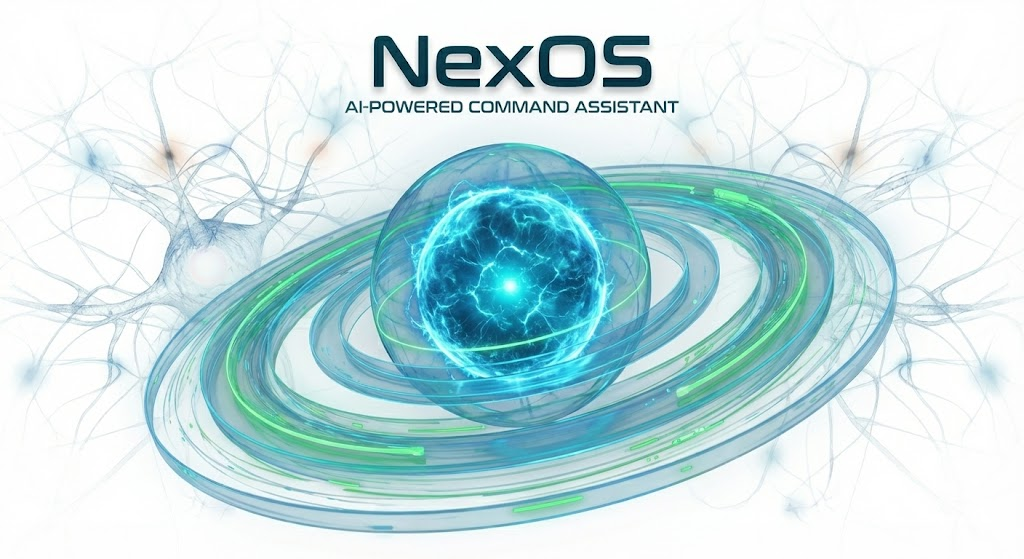
\includegraphics[width=3cm]{nexos_cover.png}}

\begin{document}

% -----------------------------------------------------------------------------
% SLIDE 1: KAPAK
% -----------------------------------------------------------------------------
\begin{frame}
    \titlepage
\end{frame}

% -----------------------------------------------------------------------------
% SLIDE 2: ICERIK
% -----------------------------------------------------------------------------
\begin{frame}{Sunum İçeriği}
    \tableofcontents
\end{frame}

% -----------------------------------------------------------------------------
% SLIDE 3: GIRIS
% -----------------------------------------------------------------------------
\section{Proje Tanımı ve Amaç}
\begin{frame}{NexOS Nedir?}
    \textbf{NexOS}, modern işletim sistemi kavramlarını uygulamalı olarak gösteren, Linux üzerinde çalışan eğitim amaçlı bir \textit{sanal işletim sistemi katmanıdır}.
    
    \vspace{0.5cm}
    
    \begin{columns}
        \column{0.5\textwidth}
            \textbf{Temel Özellikler:}
            \begin{itemize}
                \item Simüle edilmiş Süreç Yönetimi
                \item İzole Bellek Alanları (Sanallaştırma)
                \item Round-Robin Zamanlayıcı
                \item Sanal Dosya Sistemi
            \end{itemize}
            
        \column{0.5\textwidth}
            \textbf{Gelişmiş Özellikler:}
            \begin{itemize}
                \item AI Destekli Komut Asistanı
                \item Entegre Web Sunucu
                \item Detaylı Log Analizi
                \item Bootable ISO (Live OS)
            \end{itemize}
    \end{columns}
\end{frame}

% -----------------------------------------------------------------------------
% SLIDE 4: MIMARI
% -----------------------------------------------------------------------------
\section{Sistem Mimarisi}
\begin{frame}{Katmanlı Mimari Yapısı}
    \centering
    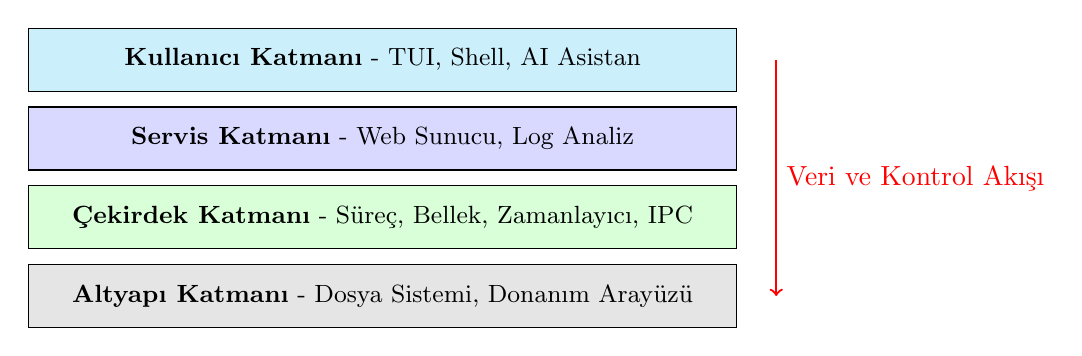
\begin{tikzpicture}[
        layer/.style={rectangle, draw, minimum width=9cm, minimum height=0.8cm, align=center, font=\small}
    ]
        \node[layer, fill=cyan!20] at (0,3) {\textbf{Kullanıcı Katmanı} - TUI, Shell, AI Asistan};
        \node[layer, fill=blue!15] at (0,2) {\textbf{Servis Katmanı} - Web Sunucu, Log Analiz};
        \node[layer, fill=green!15] at (0,1) {\textbf{Çekirdek Katmanı} - Süreç, Bellek, Zamanlayıcı, IPC};
        \node[layer, fill=gray!20] at (0,0) {\textbf{Altyapı Katmanı} - Dosya Sistemi, Donanım Arayüzü};
        
        \draw[->, thick, red] (5,3) -- (5,0) node[midway, right] {Veri ve Kontrol Akışı};
    \end{tikzpicture}
    
    \vspace{0.5cm}
    
    \begin{itemize}
        \item Modüler Yapı (C Dili)
        \item \texttt{globals.h} üzerinden merkezi veri yönetimi
    \end{itemize}
\end{frame}

% -----------------------------------------------------------------------------
% SLIDE 5: SUREC YONETIMI
% -----------------------------------------------------------------------------
\section{Çekirdek Fonksiyonları}
\begin{frame}{Süreç Yönetimi ve Durumlar}
    Her süreç 5 temel durumdan geçer:
    
    \vspace{0.5cm}
    \centering
    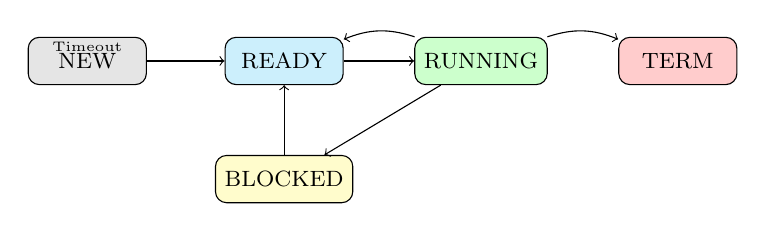
\begin{tikzpicture}[node distance=2.5cm, auto,
        state/.style={rectangle, draw, rounded corners, minimum width=1.5cm, minimum height=0.6cm, align=center, font=\footnotesize}]
        
        \node[state, fill=gray!20] (new) {NEW};
        \node[state, fill=cyan!20, right of=new] (ready) {READY};
        \node[state, fill=green!20, right of=ready] (running) {RUNNING};
        \node[state, fill=red!20, right of=running] (term) {TERM};
        \node[state, fill=yellow!20, below of=ready, node distance=1.5cm] (blocked) {BLOCKED};
        
        \draw[->] (new) -- (ready);
        \draw[->] (ready) -- (running);
        \draw[->] (running) to[bend left=20] (term);
        \draw[->] (running) to[bend right=20] (ready) node[midway, above, font=\tiny] {Timeout};
        \draw[->] (running) -- (blocked);
        \draw[->] (blocked) -- (ready);
        
    \end{tikzpicture}
    
    \vspace{0.5cm}
    \begin{itemize}
        \item \textbf{PCB (Process Control Block):} PID, Öncelik, Bellek Limiti
        \item \textbf{Zamanlayıcı:} Round-Robin (Time Quantum = 3 tick)
    \end{itemize}
\end{frame}

% -----------------------------------------------------------------------------
% SLIDE 6: BELLEK VE IPC
% -----------------------------------------------------------------------------
\begin{frame}{Bellek Yönetimi ve IPC}
    \begin{columns}
        \column{0.5\textwidth}
            \textbf{Bellek İzolasyonu}
            \begin{itemize}
                \item Her sürece özel 4KB alan
                \item Sınır kontrolü (Bounds Checking)
                \item Hatalı erişimde: \texttt{Segmentation Fault} simülasyonu ve süreç sonlandırma
            \end{itemize}
            
        \column{0.5\textwidth}
            \textbf{Süreçler Arası İletişim (IPC)}
            \begin{itemize}
                \item Mesaj Kutusu (Mailbox) mimarisi
                \item Asenkron mesajlaşma
                \item \texttt{ipc\_send} ve \texttt{ipc\_receive} fonksiyonları
            \end{itemize}
    \end{columns}
\end{frame}

% -----------------------------------------------------------------------------
% SLIDE 7: YAPAY ZEKA
% -----------------------------------------------------------------------------
\section{Yapay Zeka}
\begin{frame}{AI Entegrasyonu (Ollama + Qwen)}
    \begin{columns}
        \column{0.6\textwidth}
            NexOS, kullanıcıya komut satırında yardımcı olan bir \textbf{AI Asistan} içerir.
            
            \vspace{0.3cm}
            \textbf{Teknolojiler:}
            \begin{itemize}
                \item \textbf{Motor:} Ollama (Local LLM Runtime)
                \item \textbf{Model:} Qwen 1.5B (Fine-tuned)
                \item \textbf{Dataset:} BusyBox komut seti
            \end{itemize}
            
            \vspace{0.3cm}
            \textit{"İnternet gerektirmez, tamamen yerel çalışır."}
            
        \column{0.4\textwidth}
            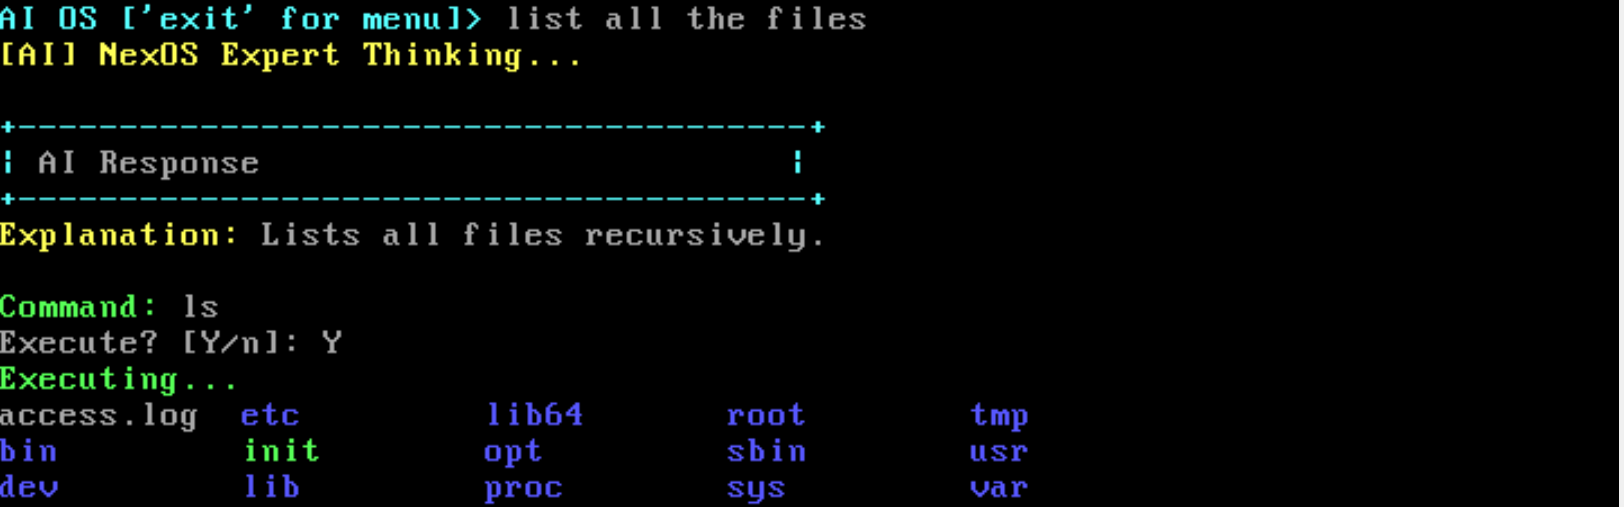
\includegraphics[width=\textwidth]{images/airesponse.PNG}
    \end{columns}
\end{frame}

% -----------------------------------------------------------------------------
% SLIDE 8: LOG ANALIZ VE WEB
% -----------------------------------------------------------------------------
\section{Servisler}
\begin{frame}{Log Analizi ve Web Sunucu}
    \begin{columns}
        \column{0.5\textwidth}
            \textbf{Log Analiz Modülü}
            \begin{itemize}
                \item \texttt{awk}, \texttt{sort}, \texttt{uniq} ile veri madenciliği
                \item Saldırı tespiti (SQLi, XSS, Path Traversal)
                \item Otomatik HTML raporlama
            \end{itemize}
            
        \column{0.5\textwidth}
            \textbf{Web Sunucu}
            \begin{itemize}
                \item BusyBox \texttt{httpd} altyapısı
                \item Dinamik Dashboard
                \item Basic Authentication
                \item Canlı sistem izleme
            \end{itemize}
    \end{columns}
\end{frame}

% -----------------------------------------------------------------------------
% SLIDE 9: DEMO
% -----------------------------------------------------------------------------
\section{Demo Görüntüleri}
\begin{frame}{Kullanıcı Arayüzü (TUI)}
    \centering
    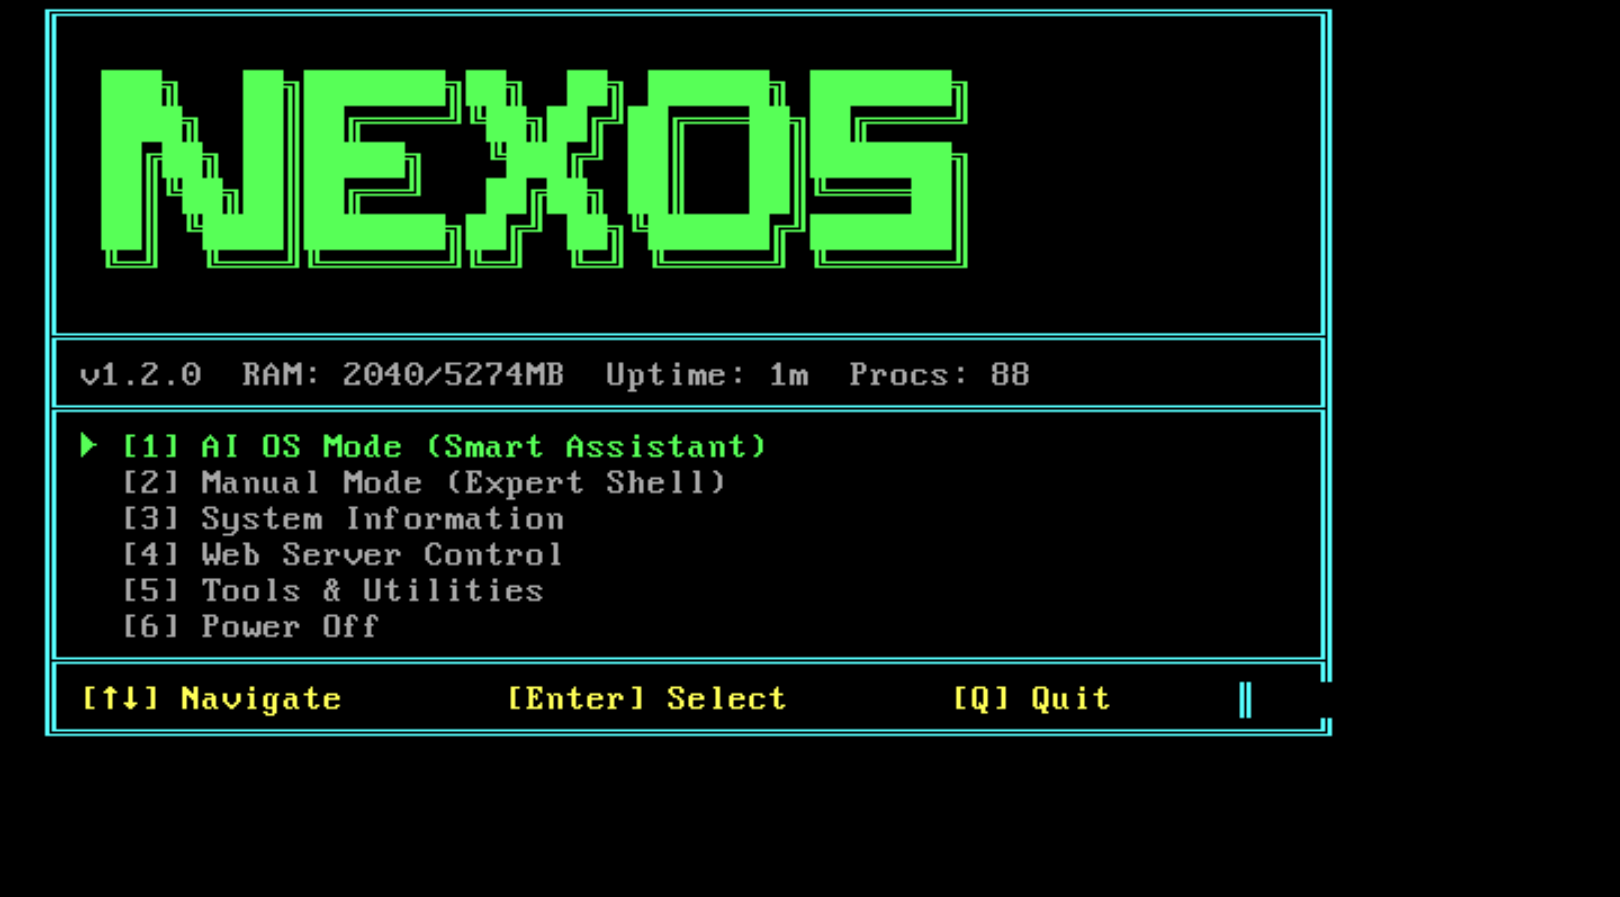
\includegraphics[width=0.75\textwidth]{images/dashboard.PNG}
    
    \vspace{0.2cm}
    \textit{Ana Ekran ve Sistem Özeti}
\end{frame}

\begin{frame}{Sistem İzleme}
    \centering
    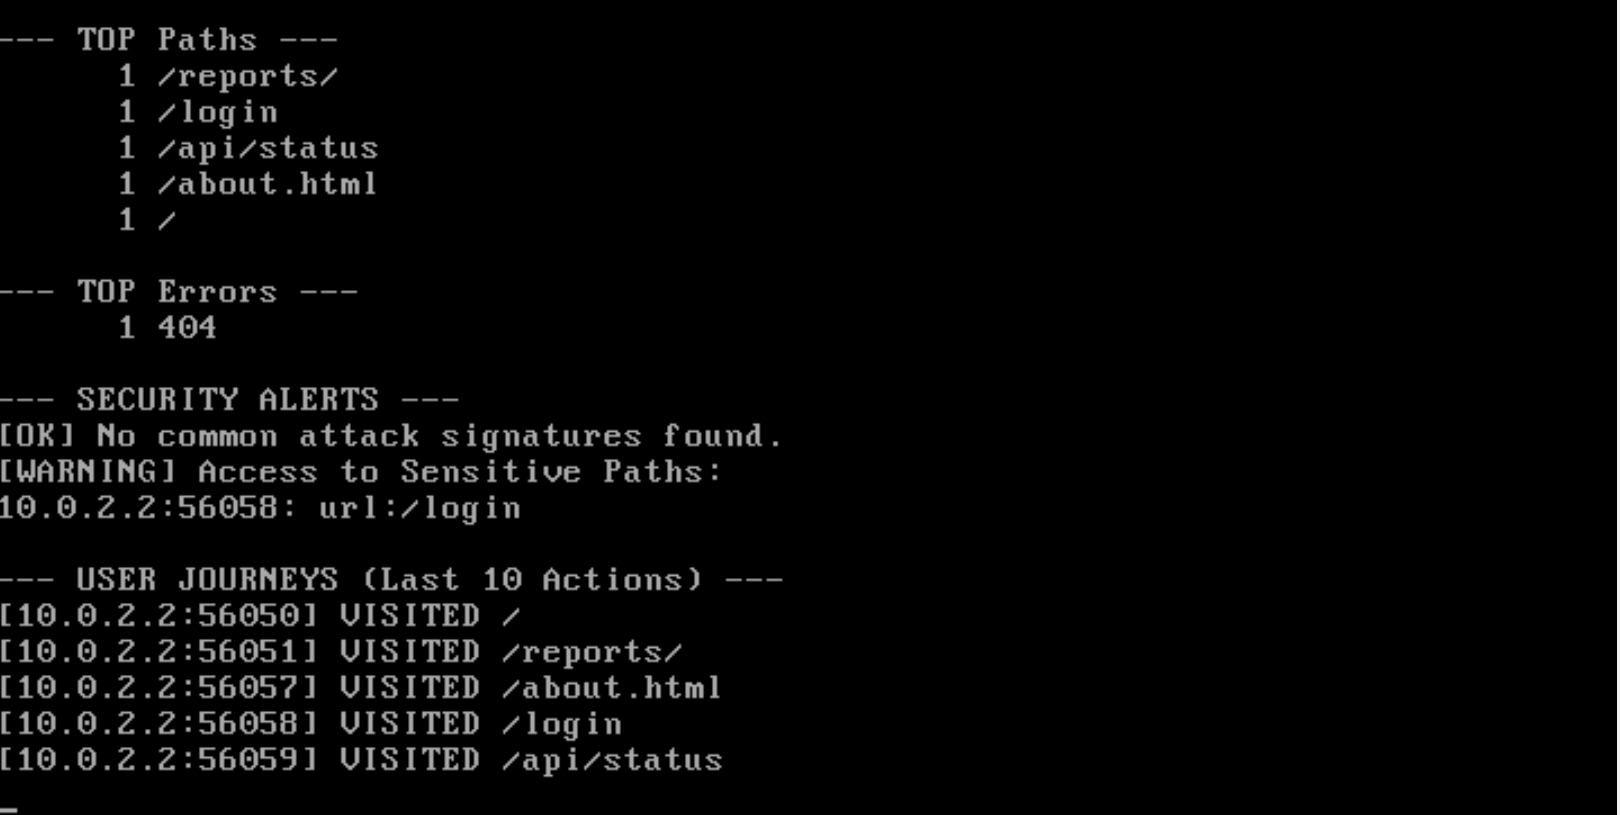
\includegraphics[width=0.75\textwidth]{images/monitor.PNG}
    
    \vspace{0.2cm}
    \textit{Canlı Kaynak Tüketimi}
\end{frame}

% -----------------------------------------------------------------------------
% SLIDE 10: SONUC
% -----------------------------------------------------------------------------
\section{Sonuç}
\begin{frame}{Proje Kazanımları}
    \begin{enumerate}
        \item \textbf{Sistem Programlama:} C ile kernel düzeyi simülasyon
        \item \textbf{Yapay Zeka:} LLM entegrasyonu ve fine-tuning
        \item \textbf{Linux Yetkinliği:} Scripting, ISO oluşturma, Boot süreci
        \item \textbf{Güvenlik:} Bellek izolasyonu ve Log analizi
    \end{enumerate}
    
    \vspace{1cm}
    \centering
    \Large \textbf{TEŞEKKÜRLER}
\end{frame}

\end{document}
